\begin{figure}[H]
\centering
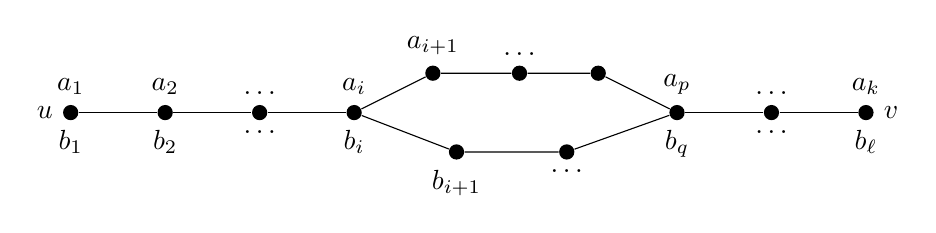
\begin{tikzpicture}[
  dot/.style={circle, fill=black, inner sep=0pt, minimum size=5.5pt},
  node distance=1.3cm
]
  % Left linear path
  \node[dot, label=left:$u$, label=above:$a_1$, label=below:$b_1$] (u) at (0,0) {};
  \node[dot, label=above:$a_2$, label=below:$b_2$] (v2) at (1.2,0) {};
  \node[dot, label=above:$\dots$, label=below:$\dots$] (v3) at (2.4,0) {};
  \node[dot, label=above:$a_i$, label=below:$b_i$] (ai) at (3.6,0) {};

  % Top cycle branch
  \node[dot, label=above:$a_{i+1}$] (top1) at (4.6, 0.5) {};
  \node[dot, label=above:$\dots$] (top2) at (5.7, 0.5) {};
  \node[dot] (top3) at (6.7, 0.5) {};

  % Bottom cycle branch
  \node[dot, label=below:$b_{i+1}$] (bot1) at (4.9, -0.5) {};
  \node[dot, label=below:$\dots$] (bot2) at (6.3, -0.5) {};

  % Junction node (ap / bq)
  \node[dot, label=above:$a_p$, label=below:$b_q$] (ap) at (7.7,0) {};

  % Right linear path
  \node[dot, label=above:$\dots$, label=below:$\dots$] (v11) at (8.9,0) {};
  \node[dot, label=right:$v$, label=above:$a_k$, label=below:$b_\ell$] (v) at (10.1,0) {};

  % Draw edges
  \draw (u) -- (v2) -- (v3) -- (ai);
  \draw (ai) -- (top1) -- (top2) -- (top3) -- (ap);
  \draw (ai) -- (bot1) -- (bot2) -- (ap);
  \draw (ap) -- (v11) -- (v);

\end{tikzpicture}
\end{figure}
